\documentclass[a4paper,12pt]{article}
\usepackage{polski}
\usepackage[utf8]{inputenc}
\usepackage{pdfpages}
\author{Marcin Fabrykowski}
\title{Ledicator - oświetlenie komputera wykonane w technologii led}
\begin{document}
\maketitle
\newpage
\tableofcontents
\newpage
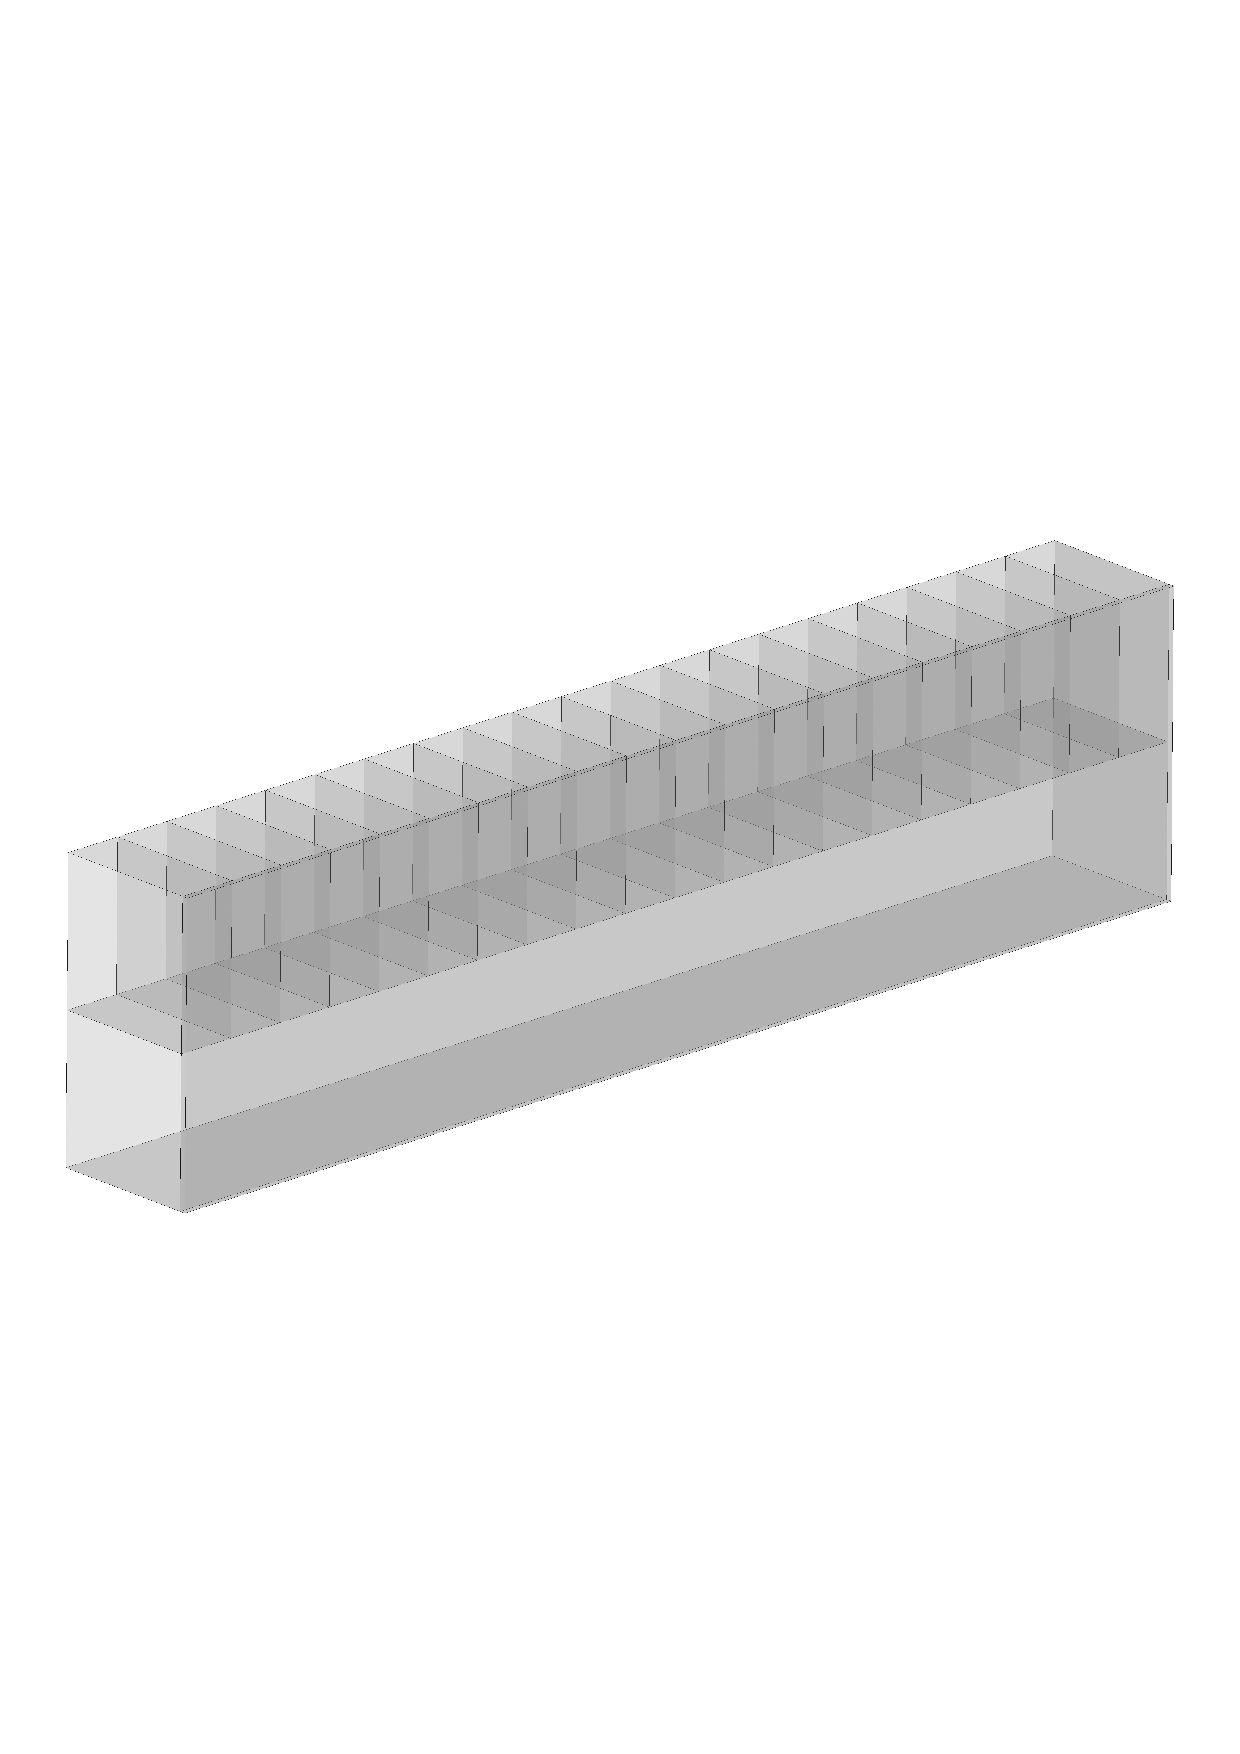
\includepdf{print.pdf}
\section{Opis produktu}
	Przedmiotem opracowania jest sterowalny wskaźnik wykonany w~technologii led.
	Urządzenie podłączane jest do komputera za pomocą portu USB.
	
	Wykonane zostanie z~wykorzystaniem 20 diod led.
	Zamontowane zostaną trzy rodzaje diod:
	\begin{itemize}
		\item diody zielone: 10 szt
		\item diody żółte: 5 szt
		\item diody czerwone: 5 szt
	\end{itemize}
	
	Całość zostanie zabudowana w~2 mm, bezbarwną płytę plexi. Pozwoli to na oglądanie zamieszczonej wewnątrz elektroniki.

\section{Dane techniczne}
	\begin{itemize}
		\item Napięcie zasilania: 5V DC
		\item Złącze: USB
		\item Pobór prądu: 20x 10mA = 200mA
	\end{itemize}
\section{Sterowanie}
	\subsection{Wysokopoziomowe}
		Sterowanie odbywa się przy użyciu programu sterującego załączonego do urządzenia na płycie CD bądź pobranego ze strony internetowej.
		Program pozwala na wybranie jednego z dostępnych schematów oświetlenia i animacji, bądź prezentowania monitorowanych wartości, takich jak obciążenie procesora, zużycie RAM bądź zajętość dysku.
	\subsection{Niskopoziomowe}
		Komunikacją z urządzeniem zajmuje się moduł jądra umieszczony na płycie CD bądź pobrany ze strony internetowej.	
		Sterowanie urządzeniem odbywa się poprzez przesyłanie wartości z przedziału od 0 do 1048576 do deskryptorów modułu obsługującego.
		Przesłana wartość jest interpretowana jako mapa bitowa, gdzie kolejne bity odpowiadają za tryb zapalenie kolejnych diod.
\section{Schemat}
	Tutaj powinny być schematy urządzenia.
\section{Kosztorys}
	\begin{tabular}{|l|c|}
	\hline
	\textbf{Nazwa}&\textbf{cena}\\
	\hline
	Płytka drukowana (100x20 mm)&4 PLN\\
	Płyta plexi(2x 240x25 + 2x 240x50 + 2x 25x50)&1.5 PLN\\
	Diody (20x)&2.8 PLN\\
	Kabel USB&4 PLN\\
	Elektronika (do zaprojektowania)& ok 10 PLN\\
	\hline
	Suma:&22.3 PLN\\
	\hline
	\end{tabular}
\newpage
\section{Instrukcja obsługi}
	\begin{enumerate}
		\item Podłączyć urządzenie do komputera
		\item Skompilować i~zainstalować moduły:
			\begin{verbatim}
			cd /mnt/cdrom/modules
			make
			make install
			\end{verbatim}
			gdzie \textit{/mnt/cdrom} jest punktem montowania płyty CD
		\item Załadować moduł jądra:
			\begin{verbatim}
			modprobe ledicator.ko
			\end{verbatim}
		\item Uruchomić program sterujący:
			\begin{verbatim}
			/mnt/cdrom/apps/ledicator
			\end{verbatim}
		\item Wybrać schemat działania zgodnie z indywidualnymi preferencjami
	\end{enumerate}
\end{document}
